\documentclass{article}
\usepackage[utf8]{inputenc}
\usepackage[T1]{fontenc}
\usepackage{graphicx}
\usepackage{hyperref}
\usepackage{geometry}
\geometry{margin=1in}

\title{BUTTRESS}
\date{Encyclopaedia Britannica (1771)}

\begin{document}
\maketitle

\section*{Historical source}
\textbf{Entry ID:} \texttt{entry-buttress-2250} \\
\textbf{Volume ID:} 144133901 \\
\textbf{Character Count:} 685

\subsection*{Extracted Text}
BUTTRESS, a kind of batment built archwife, or a mals of flouse or birds, ferving to prop of flapper the fides of a building, wall, 6e, on the outside, where it is either very high, or has any considerable load to fultain on the other fide, as a bank of earth, eC Butteflies are used against the angles of fleeples and other buildings of flone, 6e, on the confiile, and along the walls of fuch buildings at have great and heavy roofs, which would be subject to shrull the walls once, unless very thick, if no butteffes were placed againft them. They are also placed for a lupport and bammer against the feet of fine arches, that are turned around great halls in old palaces, abbys, cz.



\section*{Source record}
\begin{itemize}
\item \textbf{Dataset:} \texttt{NationalLibraryOfScotland/encyclopaedia\_britannica\_illustrated}
\item \textbf{Dataset Revision:} \texttt{309f765b1ecc83e0a7f7762e44b4a927a7555443}
\item \textbf{Page ID:} \texttt{britannica:309f765b1ecc83e0a7f7762e44b4a927a7555443:train:2250} \\
  \textbf{Filename:} \texttt{page-2250-75315f455009.jpg} \\
  \textbf{Row Index:} 2250 \\
  \textbf{SHA256:} \texttt{75315f45500988da...}
\end{itemize}

\begin{figure}[h]
\centering
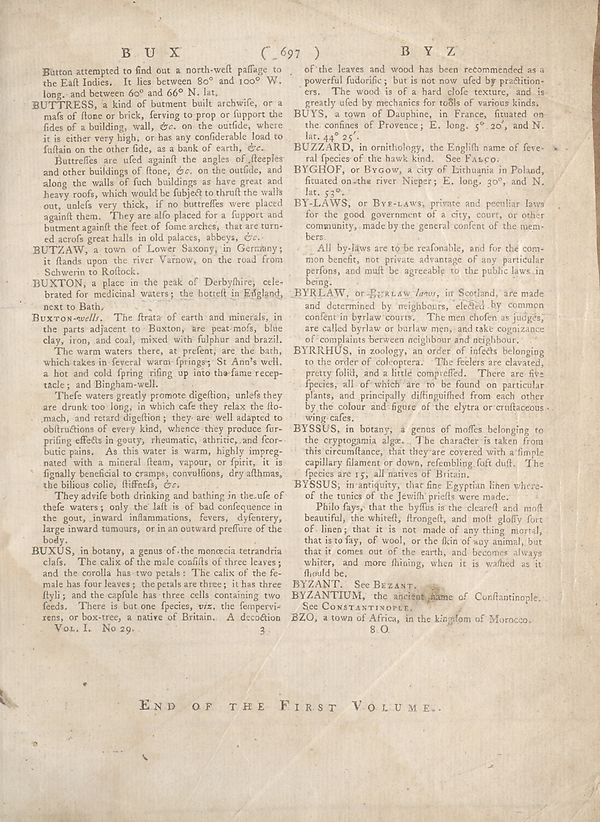
\includegraphics[width=0.85\textwidth]{../scans/page-2250-75315f455009.jpg}
\caption*{Source scan: \texttt{page-2250-75315f455009.jpg}}
\end{figure}

\end{document}
